\section{Algorithms for Gradient-Based Optimization}

Most neural network learning rules have their roots in statistical correlation analysis and
in gradient descent search procedures. The objective is to find a set of parameters $\theta$ that minimizes a predefined cost or loss function J($\theta$). The cost function is a quantitative measure of how much there is a discrepancy between the predicted output of the neural network and the ground truth or target values over a dataset.

For a network with a high-dimensional parameter space, an analytical solution for minimizing J($\theta$) is intractable. Consequently, iterative numerical optimization methods are employed.

\subsection{Gradient Descent}

The core principle behind gradient descent is to utilize the gradient ∇J($\theta$) that indicates the direction of the steepest ascent of the cost function. By moving in the opposite direction of the gradient, we can iteratively update the parameters to reduce the cost function.

we express that as :
\[
\theta_{new} = \theta_{old} - \eta \nabla J(\theta_{old})
\]

where $\eta$ is the learning rate, a hyperparameter that controls the step size of each update.




\begin{figure}[h]
	\centering
	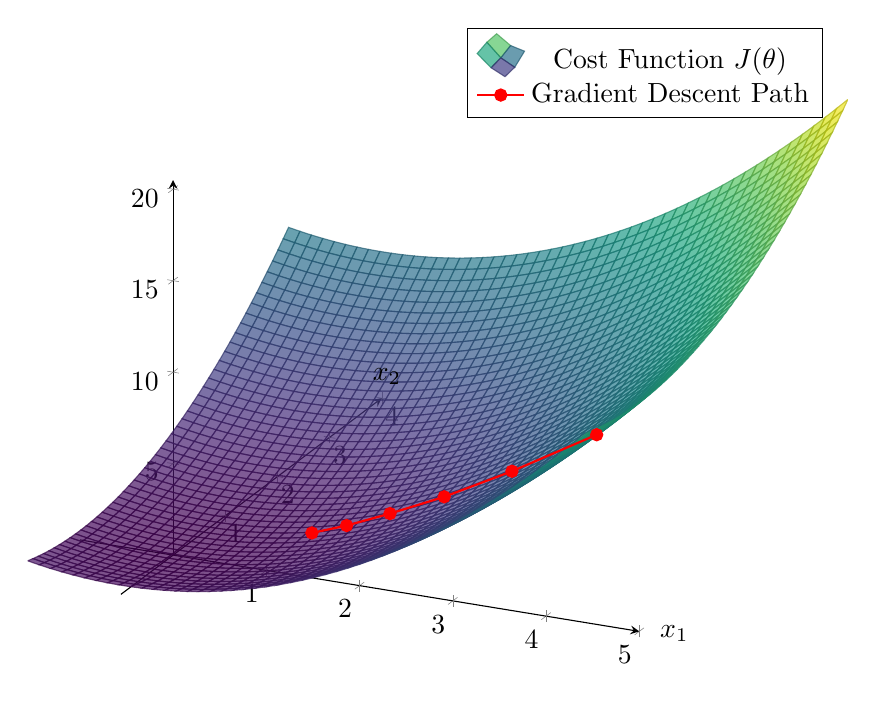
\begin{tikzpicture}
		\begin{axis}[
			width=12cm,
			height=10cm,
			axis lines=middle,
			xlabel={$x_1$},
			ylabel={$x_2$},
			xmin=-1, xmax=5,
			ymin=-1, ymax=4,
			xtick={0,1,2,3,4,5},
			ytick={0,1,2,3,4},
			grid=major,
			grid style={dashed, gray!30},
			legend pos=north east,
			every axis x label/.style={at={(ticklabel* cs:1.02)}, anchor=west},
			every axis y label/.style={at={(ticklabel* cs:1.02)}, anchor=south},
			]
			
			% Define the cost function
			\addplot3[
			domain=-1:5,
			domain y=-1:4,
			samples=50,
			samples y=50,
			surf,
			colormap/viridis,
			opacity=0.7,
			] {0.5*(x^2 + y^2)};
			\addlegendentry{Cost Function $J(\theta)$}
			% Gradient descent path
			\addplot3[
			thick,
			color=red,
			mark=*,
			mark options={fill=red},
			] coordinates {
				(3.2,2.4,4.1)
				(2.56,1.92,2.6)
				(2.048,1.536,1.6)
				(1.6384,1.2288,1.0)
				(1.31072,0.98304,0.6)
				(1.048576,0.786432,0.4)
			};
			\addlegendentry{Gradient Descent Path}
		\end{axis}
	\end{tikzpicture}
	\caption{Illustration of Gradient Descent on a 3D Cost Function Surface}
	\label{fig:gradient_descent}
\end{figure}

\subsection{Variants of Gradient Descent}

The primary problem with standard gradient descent is that it requires computing the gradient over the entire dataset, (which is known as \textit{batch gradient descent}), which can be computationally expensive for large datasets. To address this, several variants of gradient descent have been developed:

\begin{itemize}
	\item \textbf{Stochastic Gradient Descent (SGD):} Instead of computing the gradient over the entire dataset, SGD uses an istimation of the gradient based on a small, randomly sampled subset of the training data (which is know as a \textit{mini-batch}).
	instead of comupting a full loss J($\theta$) over the entire dataset, we uses a an approximation over a mini-batch of size m:
	\[
	J_{m}(\theta) = \frac{1}{m} \ \sum_{i=1}^{m} L(y_i, f(x_i; \theta))
	\]
	
	and this offers an unbiased estimate of the true gradient:
	\[\nabla J_{m}(\theta) \approx \nabla J(\theta)\]
	Yet this gradient suffers from high noise, which can lead to oscillations in the parameter updates. However, this noise can also help the optimization process escape local minima and explore the parameter space more effectively.
	
	\item \textbf{Adaptive Optimization Algorithms :} Standard SGD can be further enhanced with techniques that adapt the learning rate during training based on the history of its gradients.
	This concept is inspired by the introduction of momentum, where instead of risking to get stuck in a local minimum, especialy if the \textit{error surface} (the surface defined by the cost function over the parameter space) has many local minima, a possible solution is using an avrage of the gradients, which is a very expensive operation. As a shortcut, that was introduced by \citep{Rumelhart1986}, is to make the weight update in the \textit{I th} iteration depend not only on the gradient at that iteration, but also on the previous weight update:
	\[
	\Delta \theta_{I} = -\eta \nabla J(\theta_{I-1}) + \alpha \Delta \theta_{I-1}
	\]
	\[
	\theta_{I} = \theta_{I-1} + \Delta \theta_{I}
	\]
	where $\alpha$ is the momentum coefficient, typically set between 0.5 and 0.9.
	
	A more refined version is the \textbf{Nesterov Accelerated Gradient (NAG)}. In NAG, the gradient is computed not at the current parameters but at the anticipated future position of the parameters:
	\[
	\Delta \theta_{I} = -\eta \nabla J(\theta_{I-1} + \alpha \Delta \theta_{I-1}) + \alpha \Delta \theta_{I-1}
	\]
	\[
	\theta_{I} = \theta_{I-1} + \Delta \theta_{I}
	\]
	
	
	\item \textbf{Per-Parameter Adaptive Learning Rates:} Algorithms like AdaGrad, RMSProp, and Adam adjust the learning rate for each parameter individually based on the historical gradients. Where the latest of them is Adam, which is the de-facto standard for training deep learning models. Adam combines the benefits of both momentum and adaptive learning rates by maintaining moving averages of both the gradients and their squared values:
	\[
	m_{t} = \beta_1 m_{t-1} + (1 - \beta_1) \nabla J(\theta_{t-1})
	\]
	\[v_{t} = \beta_2 v_{t-1} + (1 - \beta_2) (\nabla J(\theta_{t-1}))^2
	\]
	\[\hat{m}_{t} = \frac{m_{t}}{1 - \beta_1^t}
	\]
	\[\hat{v}_{t} = \frac{v_{t}}{1 - \beta_2^t}
	\]
	\[\theta_{t} = \theta_{t-1} - \eta \frac{\hat{m}_{t}}{\sqrt{\hat{v}_{t}} + \epsilon}
	\]
	where \(m_t\) and \(v_t\) are the first and second moment estimates, \(\beta_1\) and \(\beta_2\) are decay rates, and \(\epsilon\) is a small constant to prevent division by zero.
\end{itemize}


